\documentclass[10pt,a4paper]{article}
\usepackage[right=0.5cm, left=0.5cm,top=1cm,bottom=1.5cm]{geometry}
\usepackage{enumitem}
\usepackage{graphicx}
\usepackage{array, tasks}
\usepackage{blindtext}
\usepackage{fontspec}
\usepackage{amsmath,amsfonts,amssymb,mathrsfs,amsthm}
\usepackage{fancyhdr}
\usepackage{xcolor}
\usepackage{booktabs}
\usepackage[font={bf}]{caption}
% \captionsetup[table]{box=colorbox,boxcolor=orange!20}
\usepackage{float}
\usepackage{esvect}
\usepackage{tabularx}
\usepackage{pifont}
\usepackage{colortbl}
 \usepackage{fancybox}
 \mathversion{bold}
 \usepackage{pgfplots}
 % \usepackage[utf8]{inputenc}
\usepackage{tikz}
 \usepackage[tikz]{bclogo}%
 \usepackage{mathpazo}
\usepackage{ulem}
\usepackage{yagusylo}
\usepackage{textcomp}\usepackage{blindtext}
\usepackage{multicol}
\usepackage{varwidth}
\usetikzlibrary{calc,intersections}
\usepackage{pgfplots}
%\usepackage{fourier}
\pgfplotsset{compat=1.11}
\usepackage{tkz-tab}
\usepackage{xcolor}
\usepackage{color}
\usetikzlibrary{calc}
\mathchardef\times="2202
\usepackage[most]{tcolorbox}
\definecolor{lightgray}{gray}{0.9}
\definecolor{ocre}{RGB}{0,244,244} 
\definecolor{head}{RGB}{255,211,204}
\definecolor{browndark}{RGB}{105,79,56}
%\RequirePackage[framemethod=default]{mdframed}
\usepackage{tikz}
\usetikzlibrary{calc,patterns,decorations.pathmorphing,arrows.meta,decorations.markings}
\usetikzlibrary{arrows.meta}
\makeatletter
\tcbuselibrary{skins,breakable,xparse}
\tcbset{%
  save height/.code={%
    \tcbset{breakable}%
    \providecommand{#1}{2cm}%
    \def\tcb@split@start{%
      \tcb@breakat@init%
      \tcb@comp@h@page%
      \def\tcb@ch{%
        \tcbset{height=\tcb@h@page}%
        \tcbdimto#1{#1+\tcb@h@page-\tcb@natheight}%
        \immediate\write\@auxout{\string\gdef\string#1{#1}}%
        \tcb@ch%
      }%
      \tcb@drawcolorbox@standalone%
    }%
  }%
}
\newcommand{\Lim}{\displaystyle\lim}
\makeatother
\newcommand{\oij}{$\left( \text{O};\vv{i},\vv{j} , \vv{k}\right)$}
\colorlet{darkred}{red!30!black}
\newcommand{\red}[1]{\textcolor{darkred}{ #1}}
\newcommand{\rr}{\mathbb{R}}
\renewcommand{\baselinestretch}{1.2}
 \setlength{\arrayrulewidth}{1.25pt}
\usepackage{titlesec}
\usepackage{titletoc}
\usepackage{minitoc}
\usepackage{ulem}
%--------------------------------------------------------------

\usetikzlibrary{decorations.pathmorphing}
\tcbuselibrary{skins}

%%%%%%%%%%%
%-------------------------------------------------------------------------
\tcbset{
        enhanced,
        colback=white,
        boxrule=0.1pt,
        colframe=brown!10,
        fonttitle=\bfseries
       }
\definecolor{problemblue}{RGB}{100,134,158}
\definecolor{idiomsgreen}{RGB}{0,162,0}
\definecolor{exercisebgblue}{RGB}{192,232,252}
\definecolor{darkbrown}{rgb}{0.4, 0.26, 0.13}

\newcommand*{\arraycolor}[1]{\protect\leavevmode\color{#1}}
\newcolumntype{A}{>{\columncolor{blue!50!white}}c}
\newcolumntype{B}{>{\columncolor{LightGoldenrod}}c}
\newcolumntype{C}{>{\columncolor{FireBrick!50}}c}
\newcolumntype{D}{>{\columncolor{Gray!42}}c}

\newcounter{mysection}
\newcounter{mysubsection}
\newcommand{\mysection}[1]{%
    \stepcounter{mysection} % Increment the counter
    \textcolor{red}{\LARGE\themysection. #1 :}
}
\newcommand{\mysubsection}[2]{
    \stepcounter{mysubsection}
    \textcolor{red}{\large \themysection.#1. #2 :}
}
% \textcolor{red}{\LARGE\bfseries 1. Les équation du deuxiéme degrée :}

%------------------------------------------------------
\newtcolorbox[auto counter]{Definition}{enhanced,
before skip=2mm,after skip=2mm,
colback=yellow!20!white,colframe=lime,boxrule=0.2mm,
attach boxed title to top left =
    {xshift=0.6cm,yshift*=1mm-\tcboxedtitleheight},
    varwidth boxed title*=-3cm,
    boxed title style={frame code={
                        \path[fill=lime]
                            ([yshift=-1mm,xshift=-1mm]frame.north west)  
                            arc[start angle=0,end angle=180,radius=1mm]
                            ([yshift=-1mm,xshift=1mm]frame.north east)
                            arc[start angle=180,end angle=0,radius=1mm];
                        \path[left color=lime,right color = lime,
                            middle color = lime]
                            ([xshift=-2mm]frame.north west) -- ([xshift=2mm]frame.north east)
                            [rounded corners=1mm]-- ([xshift=1mm,yshift=-1mm]frame.north east) 
                            -- (frame.south east) -- (frame.south west)
                            -- ([xshift=-1mm,yshift=-1mm]frame.north west)
                            [sharp corners]-- cycle;
                            },interior engine=empty,
                    },
fonttitle=\bfseries\sffamily,
title={Définition ~\thetcbcounter}}
%------------------------------------------------------
\newtcolorbox[auto counter]{Proposition}{enhanced,
before skip=2mm,after skip=2mm,
colback=yellow!20!white,colframe=blue,boxrule=0.2mm,
attach boxed title to top left =
    {xshift=0.6cm,yshift*=1mm-\tcboxedtitleheight},
    varwidth boxed title*=-3cm,
    boxed title style={frame code={
                        \path[fill=blue]
                            ([yshift=-1mm,xshift=-1mm]frame.north west)  
                            arc[start angle=0,end angle=180,radius=1mm]
                            ([yshift=-1mm,xshift=1mm]frame.north east)
                            arc[start angle=180,end angle=0,radius=1mm];
                        \path[left color=blue,right color = blue,
                            middle color = blue]
                            ([xshift=-2mm]frame.north west) -- ([xshift=2mm]frame.north east)
                            [rounded corners=1mm]-- ([xshift=1mm,yshift=-1mm]frame.north east) 
                            -- (frame.south east) -- (frame.south west)
                            -- ([xshift=-1mm,yshift=-1mm]frame.north west)
                            [sharp corners]-- cycle;
                            },interior engine=empty,
                    },
fonttitle=\bfseries\sffamily,
title={Proposition ~\thetcbcounter}}
%------------------------------------------------------
\newtcolorbox[auto counter]{Theoreme}{enhanced,
before skip=2mm,after skip=2mm,
colback=yellow!20!white,colframe=red,boxrule=0.2mm,
attach boxed title to top left =
    {xshift=0.6cm,yshift*=1mm-\tcboxedtitleheight},
    varwidth boxed title*=-3cm,
    boxed title style={frame code={
                        \path[fill=red]
                            ([yshift=-1mm,xshift=-1mm]frame.north west)  
                            arc[start angle=0,end angle=180,radius=1mm]
                            ([yshift=-1mm,xshift=1mm]frame.north east)
                            arc[start angle=180,end angle=0,radius=1mm];
                        \path[left color=red,right color = red,
                            middle color = red]
                            ([xshift=-2mm]frame.north west) -- ([xshift=2mm]frame.north east)
                            [rounded corners=1mm]-- ([xshift=1mm,yshift=-1mm]frame.north east) 
                            -- (frame.south east) -- (frame.south west)
                            -- ([xshift=-1mm,yshift=-1mm]frame.north west)
                            [sharp corners]-- cycle;
                            },interior engine=empty,
                    },
fonttitle=\bfseries\sffamily,
title={Théorème ~\thetcbcounter}}
%------------------------------------------------------
\newtcolorbox[auto counter]{exemple}{
  % breakable,
  enhanced,
  colback=white,
  boxrule=0pt,
  arc=0pt,
  outer arc=0pt,
  title=Exemple ~\thetcbcounter,
  fonttitle=\bfseries\sffamily\large\strut,
  coltitle=problemblue,
  colbacktitle=problemblue,
  title style={
left color=exercisebgblue,
    right color=white,
    middle color=exercisebgblue  
  },
  overlay={
    \draw[line width=1pt,problemblue] (frame.south west) -- (frame.south east);
    \draw[line width=1pt,problemblue] (frame.north west) -- (frame.north east);
    \draw[line width=1pt,problemblue] (frame.south west) -- (frame.north west);
    \draw[line width=1pt,problemblue] (frame.south east) -- (frame.north east);
  }
}
%----------------------------------------------------
\newtcolorbox[auto counter]{Activite}{
  % breakable,
  enhanced,
  colback=white,
  boxrule=0pt,
  arc=0pt,
  outer arc=0pt,
  title=Activité ~\thetcbcounter,
  fonttitle=\bfseries\sffamily\large\strut,
  coltitle=problemblue,
  colbacktitle=problemblue,
  title style={
left color=yellow!50!white,
    right color=white,
    middle color=yellow!20!white  
  },
  overlay={
    \draw[line width=1pt,problemblue] (frame.south west) -- (frame.south east);
    \draw[line width=1pt,problemblue] (frame.north west) -- (frame.north east);
    \draw[line width=1pt,problemblue] (frame.south west) -- (frame.north west);
    \draw[line width=1pt,problemblue] (frame.south east) -- (frame.north east);
  }
}
%----------------------------------------------------
\newtcolorbox[auto counter]{Application}{
  % breakable,
  enhanced,
  colback=white,
  boxrule=0pt,
  arc=0pt,
  outer arc=0pt,
  title=Application ~\thetcbcounter,
  fonttitle=\bfseries\sffamily\large\strut,
  coltitle=problemblue,
  colbacktitle=problemblue,
  title style={
left color=exercisebgblue,
    right color=white,
    middle color=exercisebgblue  
  },
  overlay={
    \draw[line width=1pt,problemblue] (frame.south west) -- (frame.south east);
    \draw[line width=1pt,problemblue] (frame.north west) -- (frame.north east);
    \draw[line width=1pt,problemblue] (frame.south west) -- (frame.north west);
    \draw[line width=1pt,problemblue] (frame.south east) -- (frame.north east);
  }
}
%----------------------------------------------------
\newtcolorbox{mybox}[2]{enhanced,breakable,
    before skip=2mm,after skip=2mm,
    colback=white,colframe=#2!30!blue,boxrule=0.3mm,rightrule=0.3mm,
    attach boxed title to top center={xshift=0cm,yshift*=1mm-\tcboxedtitleheight},
    varwidth boxed title*=-3cm,
    boxed title style={frame code={
    \path[fill=#2!30!black]
    ([yshift=-1mm,xshift=-1mm]frame.north west)
    arc[start angle=0,end angle=180,radius=1mm]
    ([yshift=-1mm,xshift=1mm]frame.north east)
    arc[start angle=180,end angle=0,radius=1mm];
    \path[draw=black,line width=1pt,left color=#2!1!white,right color=#2!1!blue!65,
    middle color=#2!1!green]
    ([xshift=-2mm]frame.north west) -- ([xshift=2mm]frame.north east)
    [rounded corners=1mm]-- ([xshift=1mm,yshift=-1mm]frame.north east)
    -- (frame.south east) -- (frame.south west)
    -- ([xshift=-1mm,yshift=-1mm]frame.north west)
    [sharp corners]-- cycle;
    },interior engine=empty,
    },
title=#1,coltitle=black,fonttitle=\sffamily}
%---------------------------------------------
\newtcolorbox{boxone}{%
    enhanced,
    colback=brown!10,
    boxrule=0pt,
    sharp corners,
    drop lifted shadow,
    frame hidden,
    fontupper=\bfseries,
    notitle,
    overlay={%
        \draw[Circle-Circle, brown!70!black, line width=2pt](frame.north west)--(frame.south west); 
        \draw[Circle-Circle, brown!70!black, line width=2pt](frame.north east)--(frame.south east);}
    }
    
\begin{document}


\begin{tcolorbox}[title=\textcolor{blue}{\shadowbox{ Prof : Othmane Laksoumi}}
\hfill
\textcolor{blue}{\shadowbox{Projection}}]
\end{tcolorbox}

\begin{mybox}{Lycée Qualifiant Zitoun}{gray}
    \begin{minipage}{8cm}
    \textcolor{darkbrown}{Année scolaire : } 2024-2025 \\
    \textcolor{darkbrown}{Niveau : } Tronc commun scientifique \\
    \textcolor{darkbrown}{Durée totale : } $5h$
    \end{minipage}
\end{mybox}

\begin{boxone}
{\Large\ding{45}}
\textcolor{red}{\large Contenus du programme :}
\begin{itemize}
    \item La projection sur une droite, la projection orthogonale, la projection sur un axe.
    \item  Théorème de Thalés : sens direct et sens réciproque.
    \item Conservation du coefficient de colinéarité de deux vecteurs.
\end{itemize}

{\Large\ding{45}}
\textcolor{red}{\large Les capacités attendues :}
\begin{itemize}
    \item Traduire vectoriellement le théorème de Thalés.
\end{itemize}

{\Large\ding{45}}
\textcolor{red}{\large Recommandations pédagogiques :} 
  \begin{itemize}
      \item On évitera toute construction théorique de la notion de projection.
      \item On rappellera le théorème de Thalés (sens directe et sens réciproque) puis on introuira, à partir d'activités, la propriété de la conservation du coefficient de colinéarité de deux vecteurs par la projection.
  \end{itemize}
\end{boxone}

\newpage

\begin{tabular}{|>{\raggedright\arraybackslash}p{17cm}|>{\centering\arraybackslash}p{0.8cm}|}
\hline
\rowcolor{head}

\centering Contenu du cours &
 Durée \\
\hline

% \vspace{1cm}
% \rotatebox{90}{Phase de lancement}

% \vspace{1cm}

% \rotatebox{90}{construction de connaissances}
 
\vspace{0.1cm}

\mysection{Projection sur une droite}
\begin{Definition}
    Soient $(D)$ et $(\Delta)$ deux droites sécantes du plan $\mathcal{P}$.
    Soit $M$ un point de $\mathcal{P}$.
    \begin{center}
        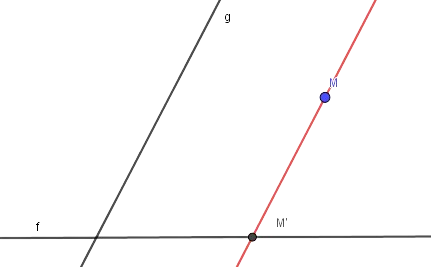
\includegraphics[width = 0.5\textwidth]{Projection1.PNG}
    \end{center}
    La droite parallèle à $(\Delta)$ et issue de $M$ coupe la droite $(D)$ en un point $M^{'}$.

    Le point $M^{'}$ est appelé \textcolor{red}{projeté} du point $M$ sur la droite $(D)$ \textcolor{red}{parallèlement} à la droite $(\Delta)$. On écrit : $p(M) = M^{'}$.

    $p$ est appelée \textcolor{red}{projection} sur $(D)$ parallèlement à $(\Delta)$.
\end{Definition}

\begin{exemple}
    On considère la figure suivante :
    \begin{center}
        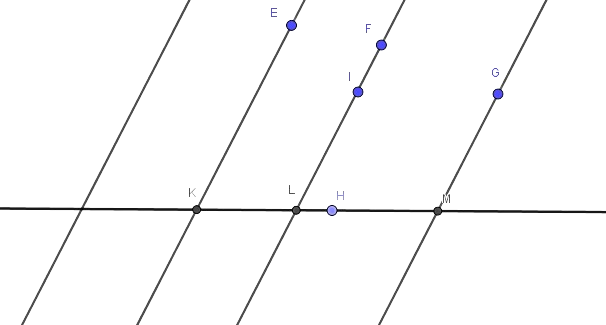
\includegraphics[width = 0.5\textwidth]{Projection2.PNG}
    \end{center}
\end{exemple}

\mysection{Projection orthogonale}
\begin{Definition}
    Soient $(D)$ et $(\Delta)$ deux droites perpondiculaires du plan $\mathcal{P}$.

    Le point $M^{'}$, projeté de $M$ sur $(D)$ parallèlement à $(\Delta)$, est appelé \textcolor{red}{projetè orthogonal} du point $M$ sur la droite $(D)$.
     \begin{center}
        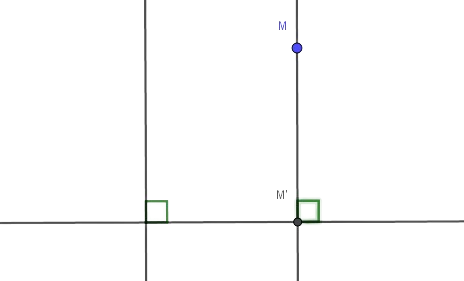
\includegraphics[width = 0.5\textwidth]{projection3.PNG }
    \end{center}
\end{Definition}



&\\
\hline

\end{tabular}




\begin{tabular}{|>{\raggedright\arraybackslash}p{17cm}|>{\centering\arraybackslash}p{0.8cm}|}
\hline
\vspace{1mm}
\begin{Proposition}
    Soient $(D)$ et $(\Delta)$ deux droites sécantes du plan.

    Le projeté de tout point de la droite $(D)$ est lui-même, par la projection sur $(D)$ parallèlement à $(\Delta)$.
\end{Proposition}

\mysection{Théorème de Thalès}
\begin{Proposition}
    Soient $(D_1)$ et $(D_2)$ deux droites sécantes en un point $A$.

    Soient $M$ et $B$ deux points de la droite $(D_1)$, distincts de $A$.
    
    Soient $N$ et $C$ deux points de la droite $(D_2)$, distincts de $A$.

    Si les deux droites $(MN)$ et $(BC)$ sont parallèles, alors : $\displaystyle\frac{AM}{AB} = \displaystyle\frac{AN}{AC} = \displaystyle\frac{MN}{BC}$
\end{Proposition}

\textcolor{red}{Remarque :}
Le thoérème de Thalès est utilisé pour calculer des longueurs.
\begin{exemple}
    Dans les trois cas suivants, on a :
   $\begin{cases}
       A,\ M,\ B \text{ sont alignés}\\
       A,\ N,\ C \text{ sont alignés}\\
       (MN) // (BC)
   \end{cases}$
   \begin{center}
       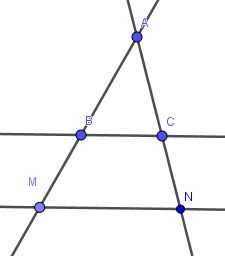
\includegraphics[width = 0.3\textwidth]{Thales1.PNG}
       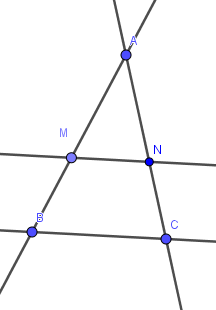
\includegraphics[width = 0.3\textwidth]{Thales2.PNG}
       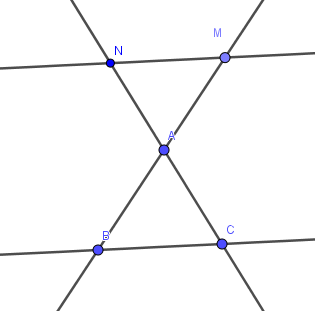
\includegraphics[width = 0.3\textwidth]{Thales3.PNG}
   \end{center}
   On en déduit : $\displaystyle\frac{AM}{AB} = \displaystyle\frac{AN}{AC} = \displaystyle\frac{MN}{BC}$
\end{exemple}
\begin{Application}
    Soit $ABC$ un triangle. Les droites $(IJ)$ et $(BC)$ sont parallèles telles que : $AI = 13$, $AJ = 5$, $AC = 39$ et $AB = x$.
    Déterminer la valeur du réel $x$.
\end{Application}

\mysection{Réciproque du théorème de Thalès}
\begin{Proposition}
    Soient $(D_1)$ et $(D_2)$ deux droites sécantes en un point $A$.

    Soient $M$ et $B$ deux points de la droite $(D_1)$, distincts de $A$.

    Soient $N$ et $C$ deux points de la droite $(D_2)$, distincts de $A$.

    Si $\displaystyle\frac{AM}{AB} = \displaystyle\frac{AN}{AC}$ et si les points $A$, $B$, $M$ et les points $A$, $C$, $N$ sont dans le même ordre, alors les droites $(MN)$ et $(BC)$ sont parallèles.
\end{Proposition}
&\\
\hline
\end{tabular}

\begin{tabular}{|>{\raggedright\arraybackslash}p{17cm}|>{\centering\arraybackslash}p{0.8cm}|}
\hline

\vspace{1mm}
\begin{Application}
    On considére la figure ci-contre tel que : 
     $\begin{cases}
        AB = 45 \\
        AC = 30 \\
        AD = 33 \\
        AE = 22
    \end{cases}$
    \newline
    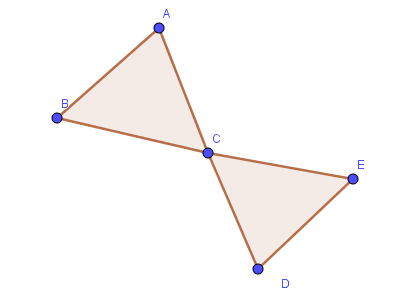
\includegraphics[width = 0.5\textwidth]{Thales4.PNG} \newline
    Montrer que : $(BC) // (DE)$.
\end{Application}

\mysection{Théorème de Thalès par la projection}
\begin{Proposition}
    Soient $(D)$ et $(L)$ deux droites.

    Soit $(\Delta)$ une droite non parallèle à $(D)$ et non parallèle à $(L)$.
    
    Soient $A,$ $B,$ $C$ des points de $(L)$ tels que $A$ et $B$ soient distincts.

    Si $A^{'},$ $B^{'},$ $C^{'}$ sont les projetés respectifs de $A,$ $B,$ $C$ sur $(D)$ parallèlement à $(\Delta)$ alors : $\displaystyle\frac{AC}{AB} = \displaystyle\frac{A^{'}C^{'}}{A^{'}B^{'}}$.

    \begin{center}
        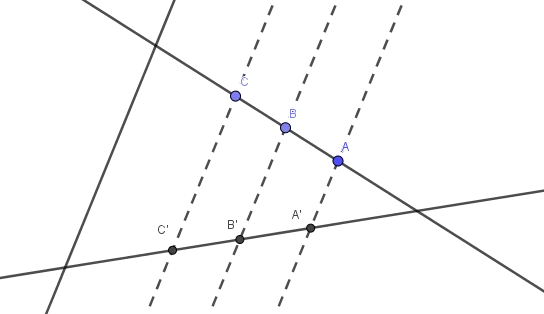
\includegraphics[width = 0.5\textwidth]{Thales5.PNG}
    \end{center}
\end{Proposition}

\mysection{Conservation du coefficient de colinéarité de deux vecteurs}
\begin{Proposition}
    Soient $(\Delta)$ et $(\Delta^{'})$ deux droites sécantes.

    Soient $\overrightarrow{AB}$ et $\overrightarrow{CD}$ deux vecteurs colinéaires tels que $\overrightarrow{CD} = k\overrightarrow{AB}$.

    Si $A^{'},$ $B^{'},$ $C^{'},$ $D^{'}$ sont les projetés respectifs des points $A,\ B,\ C$ et $D$ sur $(\Delta^{'})$ parallèlement à la droite $(\Delta),$ alors $\overrightarrow{C^{'}D^{'}} = k\overrightarrow{A^{'}B^{'}}$.
\end{Proposition}
\textcolor{red}{Remarque :}\newline
On exprime cette propriété en disant que la projection conserve le coefficient decolinéarité de deux vecteurs.

    

&\\
\hline
\end{tabular}

\begin{tabular}{|>{\raggedright\arraybackslash}p{17cm}|>{\centering\arraybackslash}p{0.8cm}|}
\hline
\vspace{1mm 
}
\begin{Application}
     Soit $ABC$ un triangle, $M$ et $N$ les points définis par :
     $$3\overrightarrow{AM} = \overrightarrow{AB}\quad \text{ et }\quad\overrightarrow{AN} + 2\overrightarrow{AB} = \overrightarrow{0}$$
     Soient $M^{'}$ et $N^{'}$ les projetés respectifs de $M$ et $N$ sur la droite $(AC)$ parallèlement à la droite $(BC)$.

     Montrer que : $\overrightarrow{MM^{'}} = \displaystyle\frac{1}{3}\overrightarrow{BC}$ et $\overrightarrow{NN^{'}} = -2\overrightarrow{BC}$
\end{Application}

&\\
\hline

\end{tabular}

\end{document} 
